\subsection{Optical pumping in rubidium }

Optical pumping is a method of driving an ensemble of atoms away from thermodynamic
equilibrium by means of the resonant absorption of light. Rubidium resonance radiation is
passed through a heated absorption cell containing rubidium metal and a buffer gas —
typically a noble gas such as neon. Without the buffer gas, rubidium atoms would quickly
collide with the walls of the cell, tending to destroy the optical pumping. Collisions with
the buffer gas are much less likely to destroy the pumping, thus allowing a greater degree
of population transfer to be obtained.
 
\subsubsection*{Apparatus Arrangement}
 
The general arrangement of the apparatus is shown in Figure~\ref{fig:op_apparatus}.
Resonance light is produced by an RF discharge lamp containing xenon gas and rubidium
metal enriched in $^{87}$Rb, excited by an oscillator operating at approximately 100~MHz.
The resonance light consists of two main lines at 780~nm and 795~nm; the 780~nm line is
removed by an interference filter, and the remaining 795~nm light is circularly polarized
before being passed through the absorption cell. A dc magnetic field is applied to the
absorption cell along the optical axis, and transitions are induced by a transverse RF
magnetic field. An optical detector monitors the intensity of the transmitted light.
 
\begin{figure}[h]
    \centering
    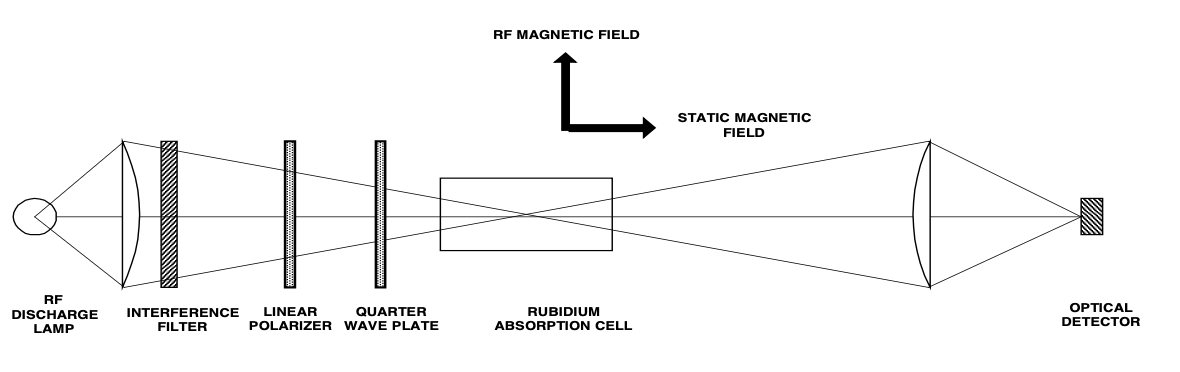
\includegraphics[width=0.7\textwidth]{theory pics/theory 2 pic.png}
    \caption{Apparatus arrangement for optical pumping.}
    \label{fig:op_apparatus}
\end{figure}
 
\subsubsection*{Pumping Mechanism}
 
The optical transitions involved in the pumping of $^{87}$Rb (nuclear spin $I = 3/2$) are
shown schematically in Figure~\ref{fig:op_transitions}. Due to the circular polarization of
the incident light, only transitions with $\Delta M = +1$ are driven. Because there is no
$M = +3$ state in the $^2P_{1/2}$ excited manifold, atoms in the $M = +2$ sublevel of the
$^2S_{1/2}$ ground state cannot absorb a photon. Atoms in all other sublevels are
optically pumped upward in $M$ and eventually decay — via spontaneous emission or
collisions — back into the ground state. Since there is a path \emph{into} the $M = +2$
level but no path \emph{out} of it via optical absorption, the population of this level
accumulates over time. This is the essence of optical pumping.
 
\begin{figure}[h] 
\centering
    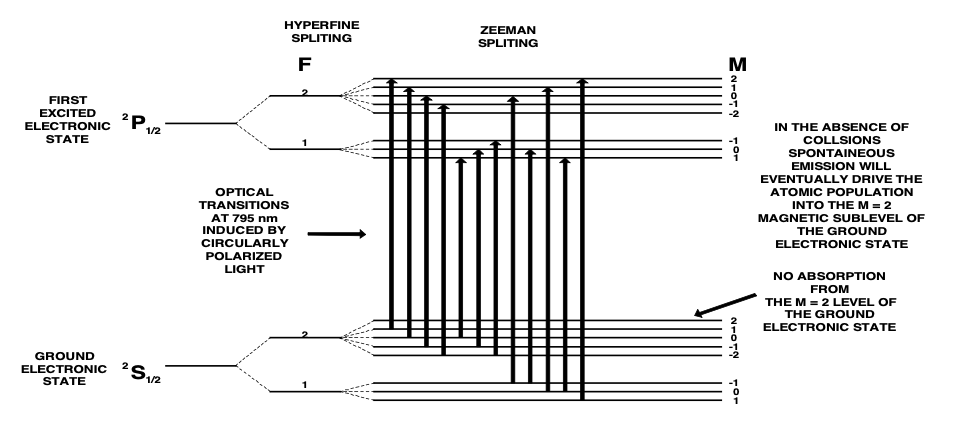
\includegraphics[width=0.65\textwidth]{theory pics/theory 3 pic.png}
    \caption{Transitions involved in the optical pumping of $^{87}$Rb ($\Delta M = +1$).
             No absorption occurs from the $M = +2$ ground sublevel.}
    \label{fig:op_transitions}
\end{figure}
 
The population of the $M = +2$ level is monitored by the intensity of the transmitted
light : any process that redistributes the population — such as RF-induced transitions
between the $M$ sublevels — will reduce the transmitted intensity. The optical pumping
process itself requires approximately 10--20~ms to achieve a suitable population in the
$M = +2$ sublevel; therefore, the rate of variation of the magnetic field must be kept
sufficiently slow.
 
\subsubsection*{Rate Equations}
 
In practice, the degree of pumping is determined by a balance between the rate of
transitions into the pumped state and the rate at which atoms are removed by collisional
relaxation. A set of rate equations describes this process. For $^{87}$Rb with nuclear spin
$I = 3/2$, there are 8 magnetic sublevels in the ground electronic state. Let $b_{ij}$ be
the probability per unit time for a transition from sublevel $i$ to sublevel $j$ due to
absorption and re-emission of a photon, and $w_{ij}$ the corresponding probability due to
relaxation processes. The occupation probability $p_k(t)$ of the $k$-th level satisfies :
\begin{equation}
    \dot{p}_k = \sum_{j=1}^{8} p_j\,(b_{jk} + w_{jk})
               - p_k \sum_{j=1}^{8} (b_{kj} + w_{kj}),
    \qquad k = 1, 2, \ldots, 8
    \label{eq:rate_eqs}
\end{equation}
with the normalization condition $\sum_k p_k = 1$, so that only seven of the eight
equations are independent.
 
It can be shown that after the pumping light is turned on, the population of the $M = +2$
(or $M = -2$) state increases exponentially in time, while the populations of the other
sublevels decrease. An excess population thus develops in the level of maximum $|M|$
compared to the thermal equilibrium distribution — this redistribution is precisely what
is meant by \textbf{optical pumping}.